%2345678901234567890123456789012345678901234567890123456789012345678901234567890
%%%%%%%%%%%%%%%%%%%%%%%%%%%%%%%%%%%%%%%%%%%%%%%%%%%%%%%%%%%%%%%%%%%%%%%%%%%%%%%%
% MAURICIO ESGUERRA NEIRA
% Ph. D. Thesis
%%%%%%%%%%%%%%%%%%%%%%%%%%%%%%%%%%%%%%%%%%%%%%%%%%%%%%%%%%%%%%%%%%%%%%%%%%%%%%%%
\chapter{Introduction}
\label{introduction} 
\bibliographystyle{nar}
\section{RNA}
RNA plays  a primordial role  in life, and  perhaps also in  the early
history   of  its   origins  \cite{woese1967,   crick1968,  orgel1968,
  orgel2004}. In Biology RNA is  a central player in the transcription
and translation steps of what is known as its central dogma, i.e., DNA
makes  RNA   (via  transcription)   and  RNA  makes   protein  (during
translation).
%A  first RNA  step  transcribes  the genetic  message
%written in the DNA alphabet, to the RNA alphabet producing mRNA.
In  the  last   decade  of  the  twentieth  century   Fire  and  Mello
\cite{fire1998} found that RNA also plays a role previously thought to
be the  job of proteins. That  is, RNA can  regulate translation using
non-coding  RNA's (ncRNA's). Another  fundamental discovery  about RNA
came  in  2000  with the  elucidation  at  atomic  level detail  of  a
non-coding   RNA,    the   ribosome   \cite{schluenzen2000,   ban2000,
  wimberly2000}.

Since its very beginnings,  structural understanding of RNA has proven
to be a very complex problem. It was not until 1956, three years after
the famous Nature triad of papers by Watson and Crick, Wilkins, Stoke,
and Wilson, and Franklin  and Gosling \cite{watson1953a} on the double
stranded structure of  DNA, that Alex Rich and  David Davies were able
to produce duble strande  RNA from polyriboadenylic acid (poly-rA) and
polyribouridylic acid  (poly-rU) to produce a  neatly difracting X-ray
pattern typical of  a double-helical structure. It was  not until 1965
that Robert Holley  was able to obtain the  complete sequence of yeast
Alanine tRNA,  and also its  secondary structure from cleavage  of the
whole structure into smaller fragments,  and it was only in 1973, that
the  first complex,  but small,  tRNA  structure, was  solved at  full
atomic detail.  Fifty seven years have passed since the description of
the  double-helical  structure  of  DNA,  but  still  RNA  faces  more
challenges  with  the  possibility  of  finding a  whole  new  zoo  of
non-coding RNA structures  \cite{weinberg2009}, and the possibility of
new engineered ones \cite{severcan2009}.

\section{Standard reference frame and local parameters}
For  the  structural  description  of RNA  the  program  \textsf{3DNA}
\cite{lu2003} has been used.  In \textsf{3DNA} there are three sets of
symmetric local parameters:
\begin{enumerate}
\item Base-pair parameters,
\item Base (base-pair) step parameters,
\item Base (base-pair) local helical parameters.
\end{enumerate}
Bases or base  pairs are treated as ``rigid  bodies'' using ideas from
classical mechanics.
%% The first two are based on cartesiancoordinates
%% (``objectcentered'', reference frame),
%% whereas the third is referred as helical coordinates
%% (non-object centered)
The first two  sets of parameters are based  on Cartesian coordinates,
whereas the  third set  of helical coordinates,  resembles cylindrical
coordinates and is based on Chasles's theorem \cite{babcock1994}.

\subsection{Base-pair and base-step parameters calculation}
In  \textsf{3DNA}   one  starts  with   a  Protein  Data   Bank  (PDB)
\cite{berman2000}  file   which  is  usually   based  on  experimental
information\footnote{This is the most common  case but the PDB file is
  sometimes  the result of  theoretical modeling.}   and which  can be
downloaded from the NDB or  PDB. This file contains the experimentally
obtained Cartesian  coordinates of  the atoms. With  this experimental
data one  performs a least-squares  fit to a standard  reference frame
\cite{olson2001}. This can be done using the \textsf{octave} script at
http://rutchem.rutgers.edu/\~{}esguerra/RNA/scripts.html as a tutorial
example.  The coordinate  origin  which is  embedded  in the  standard
reference frame is kept and used for both base and base pairs.  In the
case of  single unpaired  bases, the program  keeps the origin  of one
base of  an ideal Watson-Crick pair.  The definition of  this frame is
illustrated in Figure~\ref{fig:standard}

\begin{figure}[htbp]
\centering
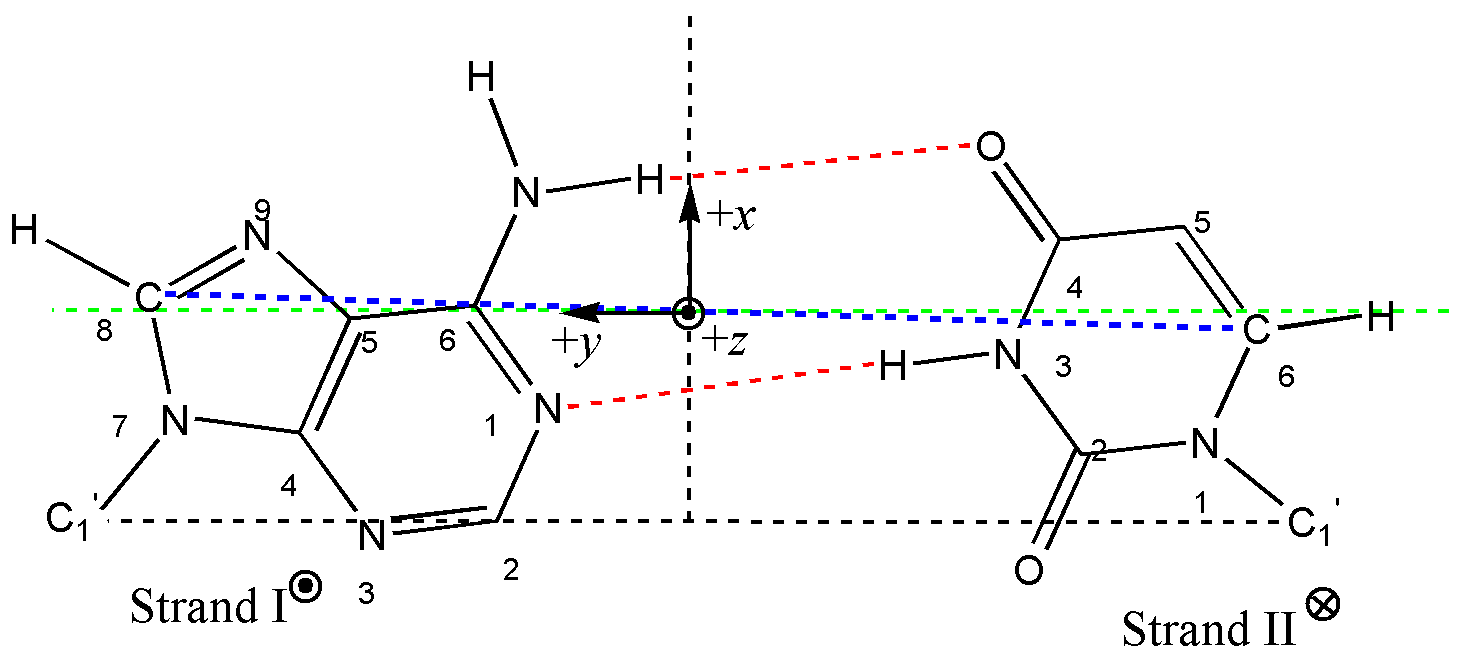
\includegraphics[scale=0.8]{Chapter1/standard.png}
\caption{Standard   reference   frame  of   an   A-T  base-pair.   The
  \textit{y}-axis (dashed green line) is  chosen to be parallel to the
  line connecting the C1$^{'}$ of  adenine and the C1$^{'}$ of thymine
  associated in  an ideal Watson-Crick  base-pair. The \textit{x}-axis
  is the perpendicular  bisector of the C1$^{'}$ -  C1$^{'}$ line, and
  the origin is located at the intersection of the \textit{x}-axis and
  the  line connecting  the C8  atom  of adenine  and the  C6 atom  of
  thymine. The  \textit{z}-axis is the cross product  of the $\hat{x}$
  and $\hat{y}$ unit vectors.}
\label{fig:standard}
\end{figure}

Once one has determined the coordinate origins for the two consecutive
bases or base pairs comprising a  step one defines a middle step triad
(MST) \cite{lu1997}. This can be described by the following procedure:

1) Find the angle $\Gamma$ between consecutive normals, \textit{i.e.},
\textit{z}-axis. Since these are unit vectors, the angle is defined by
the dot product:

\begin{gather}
\Gamma = \cos^{-1} (\hat{z}_i \cdot \hat{z}_{i+1})
\end{gather}

2)  Then find the  vector which  is perpendicular  to the  two normals
(\textit{z}-axis). This  vector is obtained from the  cross product of
the  consecutive \textit{z}-axis  (that is,  the normal  to  the plane
formed by the two vectors). This axis is called the roll-tilt axis and
is normalized to form the unit vector $\hat{r_t}$,

\begin{gather}
\hat{r_t} = \frac{\hat{z}_i \times \hat{z}_{i+1}}{|\hat{z}_i \times
\hat{z}_{i+1}|}
\end{gather}

%% Note: Why do you need a matrix? Isn't this always in 3D and therefore
%% just vectors would do? Why the more general matricial way instead of
%% the vectorial representation?
3) To make consecutive \textit{z}  vectors coincide, one uses a linear
homogeneous transformation  $R(\theta)$ about the  roll-tilt axis such
that the original orientation matrices $T_i$ and $T_{i+1}$ are rotated
by $ \theta  = \pm \Gamma / 2$ to yield  the transformed $T_i^{'}$ and
$T_{i+1}^{'}$ orientation matrices.
%% NEED to include GRAPHICS of ANGLES and COORDINATES in general.

\begin{gather}
T_i^{'} = R_{rt}(\pm \Gamma/2) T_{i} \\
T_{i+1}^{'} = R_{rt}(\mp \Gamma/2) T_{i+1}
\end{gather}

The origin  for the middle step  triad is the average  of the position
vectors for the $i$ and $i+1$ reference frames,

\begin{gather}
r_{MST} = \frac{(r_i + r_{i+1})} {2}
\end{gather}

4) Again  using the  dot product  one can find  the angle  between the
transformed  $\hat{y}^{'}$  vectors.   This  angle  is  equal  to  the
magnitude  of   the  Twist  ($\Omega$).    The  dot  product   of  the
$\hat{z}_{MST}$ unit  vector with the vector resulting  from the cross
product of $\hat{y}_{i}^{'}$ and $\hat{y}_{i+1}^{'}$ gives the sign of
$\Omega$. Since  the transformed  \textit{x-y} plane is  orthogonal to
$\hat{z}$ then this applies in the same manner for \textit{x},
%%The  vector resulting  from (yi  X yi+1  has got  to be  parallel or
%%anti-parallel to zMST, there's no other possibility.

\begin{gather}
\Omega = cos^{-1}(\hat{y}_{i}^{'} \cdot \hat{y}_{i+1}^{'})\\
(\hat{y}_{i}^{'} \times \hat{y}_{i+1}^{'}) \cdot \hat{z}_{MST} > 0, \quad \textrm{then} \ \Omega > 0\\
(\hat{y}_{i}^{'} \times \hat{y}_{i+1}^{'}) \cdot \hat{z}_{MST} < 0, \quad \textrm{then} \ \Omega < 0
\end{gather}

%%if normalized beforehand then the rule would be,
%%\begin{gather}
%%(\hat{y}_{i}^{'} \times \hat{y}_{i+1}^{'}) \cdot \hat{z}_{mst} = 1, \quad %%then \ \Omega > 1\\
%%(\hat{y}_{i}^{'} \times \hat{y}_{i+1}^{'}) \cdot \hat{z}_{mst} =
%%-1,\quad then \ \Omega < -1
%%\end{gather}

5) With more scalar product one  can find other angles, such as the phase
angle $\phi$,
%% Show in figure.

\begin{gather}
\phi = cos^{-1}(\hat{rt} \cdot \hat{y}_{MST})\\
(\hat{rt} \times \hat{y}_{MST}) \cdot \hat{z}_{MST} > 0, \quad \textrm{then} \ 180 \geq \phi \geq 0\\
(\hat{rt} \times \hat{y}_{MST}) \cdot \hat{z}_{MST} < 0, \quad \textrm{then} \ -180 \leq \phi \leq 0
\end{gather}

6) The  roll $\rho$  and tilt $\tau$  angles, which are  the remaining
angular degrees of  freedom for step parameters, are  defined in terms
of the bending angle and the phase angle:
%as if we were doing a change of variables from cartesian to polar.

\begin{gather}
\rho = \Gamma cos (\phi)\\
\tau = \Gamma sin (\phi)
\end{gather}

Now to  get the remaining  three translational degrees of  freedom for
step  parameters  ($Dx,  Dy,  Dz$)  one  just  needs  to  express  the
displacement vector in the middle step triad frame:

\begin{gather}
[D_xD_yD_z]=T_{MST}(r_{i+1} - r_{i})
\end{gather}

The  procedure  is  completely  analogous  to  compute  the  base-pair
parameters.   The  opening $\omega$,  buckle  $\kappa$, and  propeller
$\sigma$  are the  analogs of  twist $\Omega$,  roll $\rho$,  and tilt
$\tau$, and  the middle  step triad is  called middle base  triad MBT.
The axis  which are made to  coincide are the  \textit{y}-axis and not
the \textit{z}-axis as in the base-pair step case \cite{lu1997}.

The parameters obtained by  this procedure are depicted graphically in
Figure~\ref{fig:allparam}.
\begin{figure}[htbp]
\centering
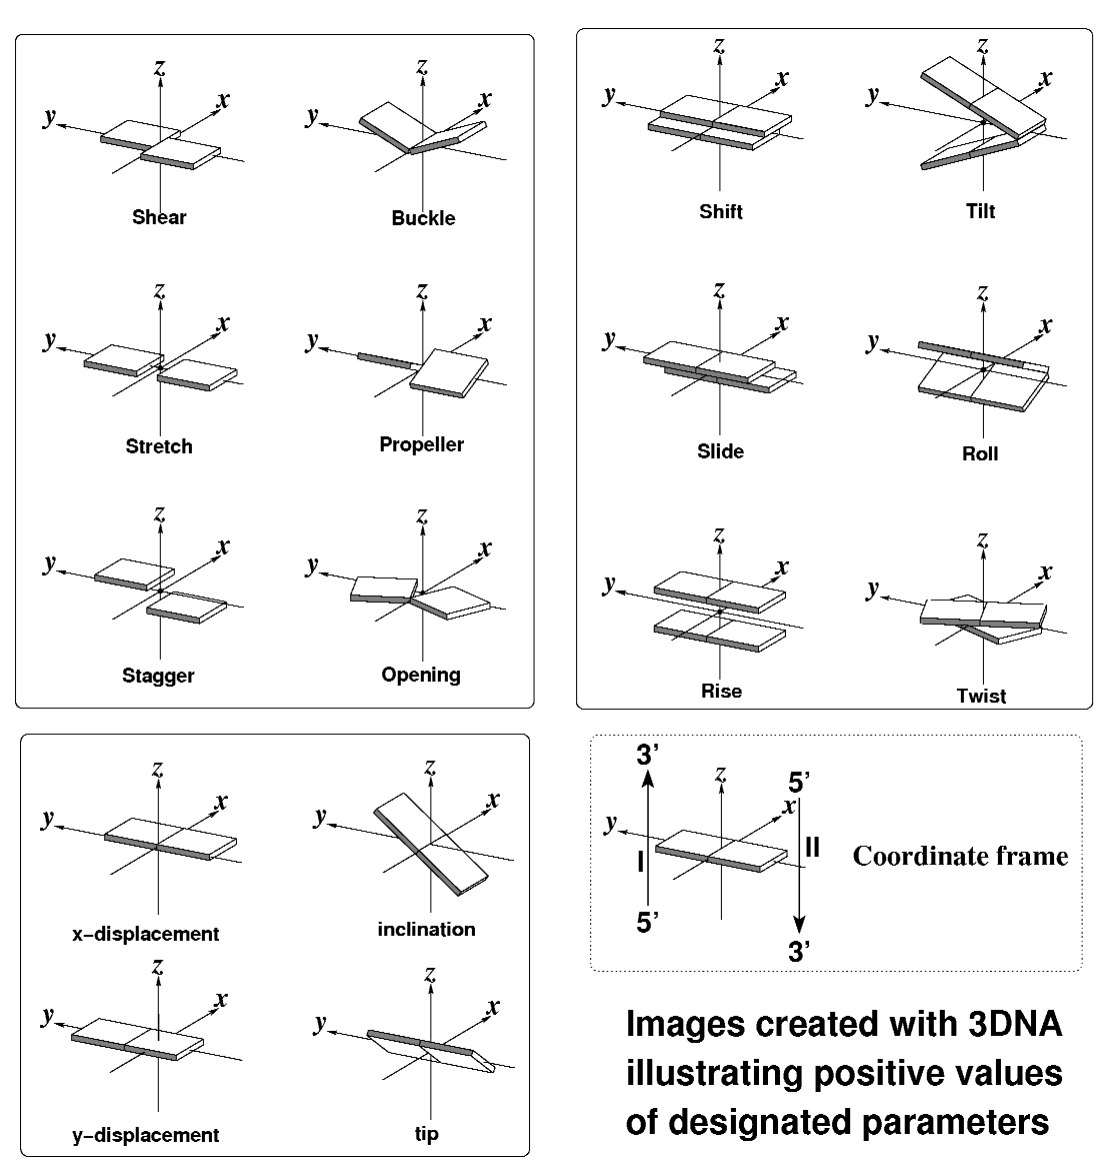
\includegraphics[scale=0.6]{Chapter1/allparam2.png}
\caption{Illustration of base pair and base step parameters \cite{lu2003}}
\label{fig:allparam}
\end{figure}


%\begin{gather}
%\gamma = \cos^{-1} (\hat{y}_{iII} \cdot \hat{y}_{iI})\\
%bo = \hat{y}_{iII} \times \hat{y}_{iI}\\
%\hat{bo} = \frac {bo}{\sqrt{bo \cdot bo}}\\
%T_{iII}^{'} = R_{bo}(+\frac{\gamma}{2}) T_{iII} \\
%_{iI}^{'} = R_{bo}(-\frac{\gamma}{2}) T_{iI}\\
%r_{mbt} = \frac{(r_{iII} + r_{iI})} {2}\\
%\omega = cos^{-1}(\hat{x}_{iII}^{'} \cdot \hat{x}_{iI}^{'})\\
%(\hat{x}_{iII}^{'} \times \hat{x}_{iI}^{'}) \cdot \hat{y}_{MBT} > 0, \quad then \ \omega > 0\\
%(\hat{x}_{iII}^{'} \times \hat{x}_{iI}^{'}) \cdot \hat{y}_{MBT} < 0, \quad then \ \omega < 0\\
%\phi^{'} = cos^{-1}(\hat{bo} \cdot \hat{x}_{MBT})\\
%(\hat{bo} \times \hat{x}_{MBT}) \cdot \hat{y}_{MBT} > 0, \quad then \ 180 \geq \phi^{'} \geq 0\\
%(\hat{bo} \times \hat{x}_{MBT}) \cdot \hat{y}_{MBT} < 0, \quad then \ -180 \leq \phi^{'} \leq 0\\
%\kappa = \gamma cos (\phi^{'})\\
%\sigma = \gamma sin (\phi^{'})\\
%[S_xS_yS_z]=T_{MBT}(r_{iI} - r_{iII})
%\end{gather}

\subsection{Local helical parameters calculation}

Local helical parameters are determined using Chasles's theorem, which
states \cite{babcock1994}:
\begin{quote}
``\textit{One can  always transport  a free rigid  body from one  position and
  orientation  to  another  position   and  orientation  by  a  single
  continuous motion along a unique axis of rotation.}''
\end{quote}

\noindent For  the three dimensional  case of nucleic acid  base steps
what   this  means   is   that,  instead   of   rotating  around   one
reference-frame  centered  axis  and  then translating  along  another
reference-frame centered  axis, one rotates about  and also translates
along   only   one  common   axis,   which   is  not   reference-frame
centered. This allows one to  define the orientation of a helical axis
(or unique  rotational-translational axis) as  a unit vector  given by
equation 2.15:

\begin{gather}
h=\left[ \begin{array}{c}
h_x\\
h_y\\
h_z
\end{array} \right]
\end{gather}
where:
\begin{gather}
h_x = \frac{\tau}{\Omega_h}, \qquad h_y = \frac{\rho}{\Omega_h},
\qquad h_z = \frac{\Omega}{\Omega_h}
\end{gather}

\begin{gather}
\Omega_h = \sqrt{\tau^2 + \rho^2 + \Omega^2}
\end{gather}

The local helical axis can be defined alternatively \cite{bansal1995}
as a cross product:

\begin{gather}
h = (x_2 - x_1) \times (y_2 - y_1)
\end{gather}
where the  $x$ and $y$ refer to  the reference frames on  base pairs 1
and 2.

\section{RNA folding}
The first  high-resolution X-ray\index{X-ray} structure  of RNA larger
than a dinucleotide was  that of yeast tRNA$^{\textrm{Phe}}$ at 3{\AA}
in  1974 \cite{robertus1974,  kim1974, stout1976}.   Thirty  six years
later there  are two orders  of magnitude more  structural information
about RNA \cite{noller2005}, and new information from non-coding RNA's
is  expected  \cite{weinberg2009}.  This  fact  and  the discovery  of
ribozymes  \cite{kruger1982,  takada1983},  which  are  catalytic  RNA
molecules, has  renewed interest in solving  the RNA folding\index{RNA
  folding}  problem,  that is,  starting  from  the primary  sequence,
finding in  an automated\footnote{The term  automated is used  here to
  mean  a  theoretical model  of  tertiary  folding,  which could  use
  experimental measures of secondary structure association in the same
  way   that  the  traditional   secondary  structure   folding  model
  \cite{zuker1989,    hofacker1994}    uses    the    Tinoco-Uhlenbeck
  dinucleotide   postulate  \cite{borer1974}   to   find  total   free
  energies.}   way the  native three-dimensional  structure of  an RNA
molecule  and   the  folding  pathway   that  it  follows.    The  RNA
folding\index{RNA folding} problem is usually seen as analogous to the
protein folding  problem, due both  to the discovery of  the enzymatic
behavior  of  RNA \cite{kruger1982,  takada1983}  and the  complicated
folding of large RNA molecules \cite{batey1999}.  To take advantage of
this analogy,  a unified conceptual  framework for describing  RNA and
protein folding, called the  kinetic partitioning mechanism (KPM), has
been developed by Thirumalai and Hyeon \cite{thirumalai2005}. This and
other methods are based on defining an adequate partition function for
describing  the correct conformational  ensemble of  folded, partially
folded,    and   unfolded    structures    \cite{chen1995,   chen1998,
  thirumalai1996} of either protein or RNA.

\section{Is RNA folding a hard or easy problem?}
There  are  two trains  of  thought  regarding  the mechanism  of  RNA
folding.  One  states that  RNA folding is  less complex  than protein
folding  \cite{tinoco1999} because  RNA is  made up  of a  four letter
alphabet of similar  nucleotide units instead of a  20 letter alphabet
of  dissimilar   amino  acids.   Therefore  the   number  of  possible
sequential  combinations  is smaller.   It  is  also  well known  that
secondary and  tertiary interactions can  be separated in the  case of
RNA  by the absence  or presence  of Mg$^{2+}$  \cite{rangan2003} (see
Figure~\ref{fig:folding}), and  that the secondary structure motifs
of RNA are more limited  in  number  than  those  of protein,  whereas
secondary  and tertiary elements are not as easily separable in
proteins.
\begin{figure}[ht]
\centering
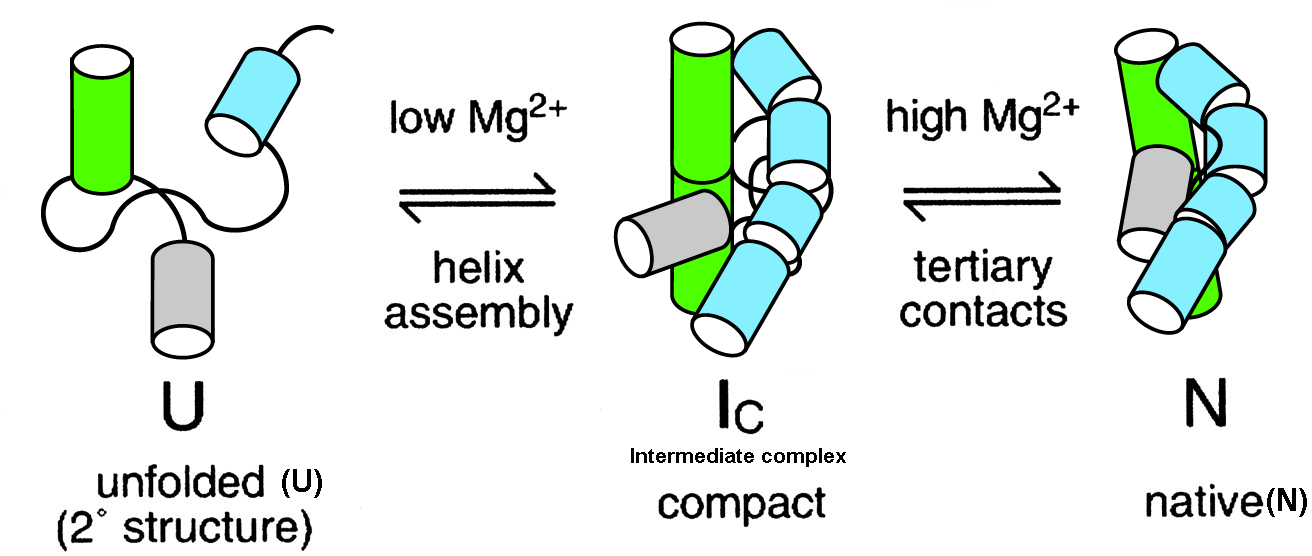
\includegraphics[scale=0.3]{Chapter1/rangan2003pnas.png}
\caption{Separation  of  secondary  and  tertiary interaction  in  RNA
  \cite{rangan2003}. Double helical secondary structure represented by
  individual  cylinders and  tertiary interactions  by  association of
  cylinders. Color coding stands for separate  helical regions of
  RNA, and the connecting  black strings represent single stranded loop
  structures.}
%% Note that Dr. Olson asks what the colors in cylinders mean.
%% Answer: They mean nothing. Perhaps only that the cyan stands for
%% the helical structures making a pseudo-knot, that is, P7 and P3.
\label{fig:folding}
\end{figure}
The  other point of  view says  that RNA  folding can  be at  least as
complex as protein folding \cite{moore1999a, sorin2004} since there is
no such thing  as hydrophobic burial of regions of RNA  as in the case
of  proteins.   Instead, the  electrostatic  problem  stemming from  a
complex charged backbone must be dealt with in the case of RNA.
% The case of the electrostatic treatment of the backbone is lacking
% here, most likely WKO wants me not to ignore our own Gerald Manning
% tinoco 1999 says this must be an easy to solve problem since we can
% do the electrostatics for it easily
For instance,  the interactions of  the RNA polyanionic  backbone with
water  and cations  \cite{klein2004a}  are not  easily simulated  with
explicit   solvent  models   like those used to treat   proteins.  The
aforementioned interactions of RNA  need to be modeled implicitly, and
must aim to describe long dynamic processes of the order of seconds to
minutes,  in  contrast   to  the  typical  time  scales   of  tens  of
microseconds associated with protein folding.
% Remember that this means that a explicit calculation for RNA would
% be prohibitively large.

Although   secondary   and  tertiary   structure   can  be   separated
experimentally, there have been few theoretical efforts to account for
the  folding  of  RNA  from  a random  sequence  of  nucleotides  into
secondary structures and tertiary  structures. What little is know has
been  investigated at  low resolution.  Stephen Harvey  and associates
have   simulated   the   folding   of   yeast   tRNA$^{\textrm{Phe}}$,
\cite{malhotra1990}  and  the  assembly  of  the 30S  subunit  of  the
ribosome \cite{stagg2003} at various levels of detail, initially using
only one pseudoatom  per helical region, and later  one pseudoatom per
nucleotide.  Recently  Fran\c{c}ois  Major's  group  at  Montreal  has
proposed a pipeline of two  computer algorithms to study RNA structure
\cite{parisien2008}.   One    pipeline   makes   secondary   structure
predictions, and the  other assembles 3D structures based  on the best
scoring secondary structures.
% Note for presentation ==> Include figure 1 in Malhotra-harvey paper
% Look at what says in folding.stanford.edu/science.html Also take
% into account Biophys J. V.88 2516-2524 for the case of having to
% think of water in the folding problem.
By contrast,  in the case of  proteins many groups  have simulated the
transition  from  secondary  to  tertiary  structure,  including  some
calculations which  account for the  strong coupling of  secondary and
tertiary  structure   \cite{westhead1999,  gerstein2003,  meiler2003}.
This type of work is  often referred to as protein structural topology
and there is no counterpart for RNA.

%The seminal paper here seems to be the one of liphardt in 2001 for
%rna unfolding
\section{Experimental folding techniques}
Traditionally   RNA   folding  and   unfolding   have  been   followed
calorimetrically  and spectroscopically as  a function  of temperature
and cation concentration  \cite{bloomfield2000, boots2008}. While this
approach  works well  for studying  two-state  folders, \textit{i.e.},
structures  which populate  only two  states (native  and  melted), in
general RNA's  are not  two-state folders. RNA  seems to go  through a
rugged  free  energy landscape  of  conformations  in  the process  of
folding \cite{zhuang2003}.  The  experimental solution to this problem
is offered  by single-molecule techniques  like fluorescence resonance
energy transfer (FRET) and  mechanical micromanipulation, in which the
ends of RNA  are attached to micron sized beads  which are then pulled
apart  and  monitored  with  a laser  light  trap  \cite{liphardt2001,
  onoa2004,  tinoco2004, hyeon2005}.  In  the case  of single-molecule
force-induced   unfolding,  state   transitions   often  occur   under
non-equilibrium  conditions, thereby  making it  difficult  to extract
equilibrium  information from the  data. Recently  Bustamante, Tinoco,
and associates have shown that by using the Crooks fluctuation theorem
\cite{crooks1999},  one  can deal  with  such  cases  and extract  RNA
folding    free     energies    from    single-molecule    experiments
\cite{collin2005}.
%\subsection{RNA Folding in Vitro vs in Vivo vs in Silico}
% It still is to be seen whether the following is relevant or not
% This single molecule information is
% collected in-vitro and not in-vivo, which is actually the ultimate
% problem aimed for prediction, there's quite a lot of evidence for
% different folding states reached in one case and not the other and
% viceversa \cite{sosnick2003, schroeder2002} but still a first step
% towards understanding in-vivo folding is in-vitro and in-silico
% experimentation.

\section{RNA simulations}
Network  and molecular  mechanics-molecular  dynamics (MM-MD)  methods
provide  useful  information  relevant  to the  RNA  folding-unfolding
problem, especially  for describing fluctuations away  from the native
conformation.   Gaussian network  models  \cite{y_wang2004, bahar1998,
  wang2005}, which  treat RNA  at less than  atomic detail,  have been
used  to  describe  the  motions  of large  RNA  structures  like  the
ribosome.  Examples  of the  predicted normal modes  of motion  of the
ribosome  can be  seen at:  http://ribosome.bb.iastate.edu/70SnK mode.
Using MM, Sanbonmatsu and coworkers  obtained a static atomic model of
the    70S    ribosome    structure    through    homology    modeling
\cite{tung2004}.  Tung  and  associates  used this  structure  for  an
all-atom  MD simulation  of the  movement of  tRNA into  a fluctuating
ribosome  \cite{sanbonmatsu2005}.  This  type of  simulation  might be
useful in a  reverse-folding approach to the RNA  folding problem.  To
the best of our knowledge,  such calculations haven't as yet been done
for RNA.

\subsection{Local nucleotide interactions}
%\subsubsection{QM approaches and MM consequences}
The molecular  interactions that  rule  RNA structures at  the nucleic
acid base level, \textit{i.e.},  local level, are hydrogen bonding and
stacking interactions. The former are  related to base pairing and the
latter, in most cases, to  nucleotide steps. These interactions can be
explored  theoretically at various  levels. At  the highest  level are
ab-initio  quantum   mechanical  calculations  which   are  still  too
expensive   for  systems  as   large  as   hundreds  of   atoms.  Such
calculations,  nevertheless,  can  tell   a  great  deal  about  local
electronic behavior.  For example, Hobza and  collaborators have found
that the  stacking interaction of free nucleotide  bases is determined
by   dispersion  attraction,   short-range  exchange   repulsion,  and
electrostatic  interaction.  No  specific $\pi-\pi$  interactions  are
found     from    electron    correlated     ab-initio    calculations
\cite{sponer1996, sponer1997}.  This is  why force field  methods have
been so successful in the  study of nucleic acids, since the empirical
potentials used  in such studies  mimic well the  quantum mechanically
obtained energy profiles \cite{tung2004, sponer2000}.
% since they can be modeled easily with simple empirical potentials
% consisting of Lennard-Jones, van der Waals and Coulomb terms.
% What the recent results say it's simply that by using a larger
% basis set, they can account for some interactions which were not
% included before, and maybe because of taking better account of
% electron-correlation.
A currently debated ab-initio finding is whether small fluctuations in
the   configurations   of   neighboring   base  pairs   (dimers)   are
iso-energetic  or  not.   Recent  calculations  of  Sponer  and  Hobza
\cite{sponer2006}    seem   to    contradict   their    earlier   work
\cite{sponer2000,  hobza2002},  in which  the  stacking energies  were
reported to  be relatively insensitive to dimer  conformation. The new
results  use  the so-called  ``coupled  cluster  singles doubles  with
triple electron excitations'' CCSD(T)  method, to account for electron
correlation.  Using  this electron correlation  energy correction, the
stacking energy differences between dimer conformations turn out to be
considerably higher than previously reported.

% therefore justifying rigid body parameter interpretations.
% \subsubsection{Experimental Stacking and Polyionic backbone}
Single-strand and double-strand stacking free energies can be obtained
calorimetrically \cite{freier1985}.   One of the  most popular methods
used   for  obtaining   such  quantities   is   differential  scanning
calorimetry (DSC) \cite{marky1982}.  These measurements show favorable
dinucleotide stacking  free energies as  large as $-3.6$  kcal/mol for
double-strand  stacking.   Experimentally,  the  magnitudes  of  these
interactions      are     found      to      be     sequence-dependent
\cite{bloomfield2000}. In  fact, the  stacking free energies  for some
sequences\footnote{Free   Energies   for   5'   unpaired   nucleotides
  (e.g. UC/A  UU/A) are quite small  (i.e.  $<$ 0.4  kcal/mol) and are
  termed  weakly stacking bases.\cite{burkard1999,  burkard1999b}} are
found to  be negligible.   Thus there may  be no  accountable stacking
interaction at all for some sequences.

Besides  taking into  account  the effects  of  stacking and  hydrogen
bonding,  it  is  important  to  think  at the  same  time  about  the
polyelectrolyte  nature  of the  RNA  backbone.  Manning's  counterion
condensation theory \cite{manning1977,  manning2003} provides a simple
and   quantitative  picture   of   the  interactions   of  a   regular
double-helical  nucleic acid  polyanion with  its counterions,  but it
does   not  take   into  account   the  discrete   nature   of  charge
\cite{bloomfield2000} or the  folding of RNA. Poisson-Boltzmann theory
offers a more detailed picture of the behavior of charged macroions in
solution \cite{antypov2005, xu2007}.
% Talk more about counterion condensation, thirumalai discusses it on
% his 2001 paper also chapter 8 of Bloomfield, Crothers, Tinoco
% (References \cite{manning2003} Ray-Manning?).
% Real Experiments results for stacking energies and polyanion
% energies and Energetics related to cation metal presence
% WKO says that there might be old experimental data that are contrary
% to this and that I must show it here, so far what I've found is
% Saenger saying that based on old QC and this is different, he
% relates it to hydrophobicity concepts. Talk about experiments.

The local conformational  space of RNA has been  studied using a large
set of available  RNA structures from the Nucleic  Acid Database (NDB)
\cite{berman1992}.  The  torsion angles  of the nucleotide  steps have
been   clustered    using   different   techniques   \cite{murray2003,
  schneider2004}.   The  root-mean-square  deviations  (RMSD)  of  the
distances between closely spaced  atoms in the phosphates, sugars, and
bases, have  also been clustered \cite{sykes2005}.  The latter studies
are aimed  at finding the  common nucleotide base steps  and base-pair
building  blocks which  have  been  given the  name  of RNA  doublets.
Recently, the  RNA Ontology Consortium (ROC) has  proposed a consensus
set  of RNA dinucleotide  conformers integrating  the work  of various
groups \cite{richardson2008}.


\subsection{RNA  secondary  structure   algorithms  and  the  lack  of
 tertiary ones}
From   secondary   structure   prediction  algorithms   like   Zuker's
\textit{mfold} program \cite{zuker2003}, Hofacker's Vienna RNA package
\cite{hofacker1994}, or  Mathews Dynaling software \cite{mathews2002},
one obtains  a large ensemble  of secondary structure graphs,  i.e. 2D
representations of  the double-stranded helical  stems, hairpin loops,
bubbles formed by the constituent bases.  These graphs can be analyzed
with graph  theory to produce  a partition function describing  a full
arrangement  of contacts for  the total  number of  possible secondary
structures, allowing  the construction  of a "relation  of microscopic
conformations to macroscopic  properties" \cite{chen2000}. So far this
type of model  has not been generalized to  take into account tertiary
structural features, \textit{i.e.},  interhelical interactions of RNA.
In  the  last  two to  three  years  a  boom  in prediction  of  small
($\approx$ 200  nucleotides) RNA 3D structures  has started. Basically
three types of approaches are being  followed.  One is that of using a
coarse-grained model, assigning a potential function to it, applying a
minimization procedure, and then performing a molecular mechanics (MM)
all-atom  refinement \cite{das2007,  ding2008,  jonikas2009a}. Another
starts  from  the predicted  secondary  structures,  assumes that  the
helical  regions adopt  the canonical  A-form  structure, mechanically
inserts residues as rigid bodies in the remaining non-helical regions,
and  finally carry  out an  MM optimization  \cite{martinez2008}.  The
third  approach   entails  a  pipeline   between  secondary  structure
prediction, and tertiary structure assembly is proposed. This pipeline
uses  as bridging  concept  between  2D and  3D  structure, the  graph
theoretical definition of a minimum cycle basis, which for the case of
nucleic  acids  has  been  renamed  as  Nucleic  Cyclic  Motifs  (NCM)
\cite{parisien2008}.

\subsection{RNA overall fold}
Whereas  in  the case  of  proteins  one  qualitatively describes  the
overall  fold  in terms  of  the  arrangement  of secondary  structure
motifs, \textit{i.e.}, using the helix-ribbon-coil images developed by
Jane           Richardson          \cite{richardson2000}          (see
Figure~\ref{fig:ribboncoil}), there is still no comparable description
of  the overall  fold of  RNA. A  ribbon representation  of  the sugar
phosphate backbone (see  Figure~\ref{fig:ribosome}) helps to understand
the  folding of  small  RNA's, but  in  the case  of  the ribosome,  a
representation at such level of detail does not allow to make sense of
such a large  structure (about 3000 nucleotides for  the large subunit
of   the  archaeal   ribosome).    In  the   past   two  years   Sykes
\cite{sykes2009}  and  Holbrook\cite{holbrook2008}  have proposed  new
representations for RNA based on helical region organization.

\begin{figure}[ht]
\centering
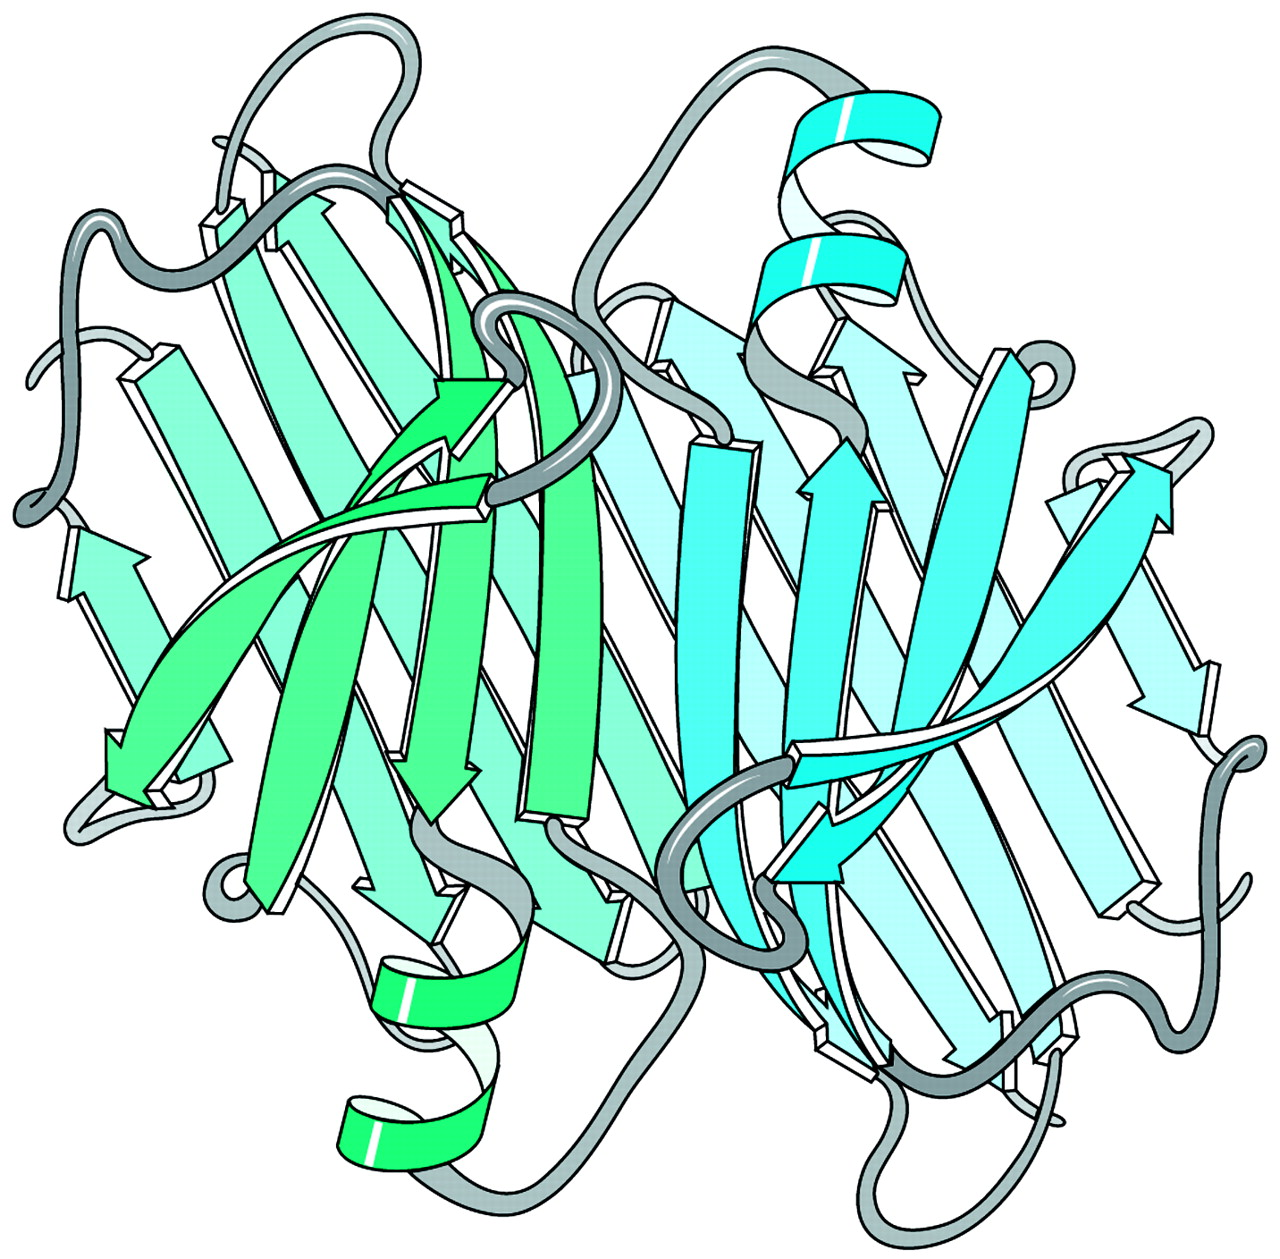
\includegraphics[scale=0.4]{Chapter1/overallfold.png}
\caption{Ribbon-coil    schematic    illustraring    the   fold    and
  intermolecular  units of  a dimer  of prealbumin  (PDB\_ID:2pab), or
  transthyretin,    taken     from    Richardson    \textit{et    al.}
  \cite{richardson2002}}
\label{fig:ribboncoil}
\end{figure}

\begin{figure}[t]
\centering
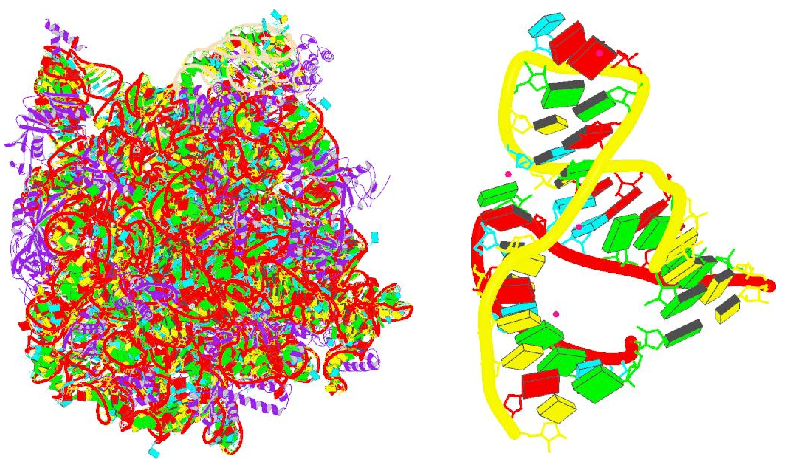
\includegraphics[scale=0.5]{Chapter1/ribosome_ribozyme.png}
\caption{\textit{Haloharcula marismortui's} large ribosomal subunit
(left) and hammerhead ribozyme (right).%NDBID:UR0029
 The figures were taken
directly from the NDB web pages, and show a ribbon
representation of the phosphate backbone, and a block representation
for the nucleotide bases. From the figures it's clear that, whereas the
ribozyme fold can be clearly understood with this representation, the
ribosome fold cannot.}
\end{figure}

One can envision that a  thorough investigation of the parameter space
of  translational and  rotational degrees  of freedom  of  the helical
regions of RNA could give clues as to how we might see an overall fold
in RNA structures.

In  the  case  of  proteins  the SCOP  (Structural  Classification  of
Proteins)  database  \cite{andreeva2004},  classifies proteins,  among
other   classifications,  according   to  recurrent   arrangements  of
secondary   structure,   that  is,   folds.    The  SCOR   (Structural
Classification of RNA) database \cite{klosterman2002, klosterman2004},
aims  to  provide  a  similar  classification  to  that  obtained  for
proteins, but using RNA motifs instead. This classification focuses on
the  local folding  of small  pieces of  RNA and  cannot  describe the
overall fold.

\subsection{RNA motifs}
First,  a word  of  caution must  be  given to  the  reader. The  term
``\textit{RNA  motif}'' alone is  used in  the literature  to describe
three   different   levels  of   RNA   organization,   that  is,   RNA
\textbf{sequence} motifs, RNA  \textbf{secondary structure} motifs, or
RNA \textbf{3D structure} motifs.  We start by making such distinction
as it is not always  clearly mentioned in RNA literature, generating a
great deal of confusion and bibliographical search frustration for the
beginner. The  kind of RNA  motifs we  are dealing with  in this
thesis are those of the third kind, that is, RNA \textbf{3D structure}
motifs  which we'll  address from  now on  simply as  RNA  motifs. Yet
another source of confusion in  understading RNA motifs is the lack of
a  unique definition. Three popular and  somewhat
recent definitions are:
\begin{itemize}
\item{RNA motifs are ``\textit{Conserved structural subunits that make
    up the secondary structures of RNAs.}''\cite{holbrook2005}}
\item{RNA   motifs    are   ``\textit{Ordered   stacked    arrays   of
    non-Watson-Crick  base  pairs  that  form distinct  folds  on  the
    phosphodiester backbones of RNA strands.}''\cite{leontis2003}}
\item{``\textit{An RNA Motif is  a discrete sequence or combination of
    base  juxtapositions   found  in  naturally   occurring  RNA's  in
    unexpectedly high abundance.}''\cite{moore1999}}
\end{itemize}
From our point of view RNA motifs are to be understood as  peculiar
sets of geometrical  (in the rigid block sense)  arrangements in three
dimensional space.

Even  though there  is no  unique definition,  we can  think  of three
practical  tasks regarding  RNA  motifs.   That is,  given  an RNA  3D
structure  automatically   identify  \cite{nasalean2009,  lemieux2006,
  duarte2003},  describe  \cite{laing2009,  laing2009a,  holbrook2008,
  spackova2006,   reblova2003},   and   find   new   \cite{sarver2008,
  mokdad2008, duarte2003, stonge2007, lemieux2006} motifs.

\section{Overview}
Keeping always in  mind the greater scope of  the RNA folding problem,
this thesis  addresses various issues of  RNA structural understanding
using RNA crystallographic data from the Protein Data Bank (PDB). Such
data  has been analyzed  statistically along  with the  use of  a very
rigourous rigid body formalism.  In Chapter 2 the consensus clustering
technique  is used to  classify RNA  base-step parameters  of non-ARNA
conformations, and  the resulting groups are  localized and understood
in the context  of rRNA.  Chapter 3 reconsiders  previous work carried
out by  Dr. Yurong Xin  at the Olson's  lab, on classification  of RNA
base-pairs by  resorting again to clustering  analysis techniques, and
database  mining  of the  WWW  available  Base  Pair Structures  (BPS)
database.  In Chapter 4  we explore,  using statistical  analysis, the
data  available on  RNA helical  regions, and  use it  to  compute the
persistence  length  of  double  stranded  RNA's  and  compare  it  to
experimental results. In  Chapter 5 we provide a  new python software,
pyRNAmotifs which  interfaces with  3DNA to do  a rigourous  search of
existing  and perhaps  new RNA  motifs, and  finally in  Chapter  6 we
propose the  measurement and classification of RNA  structures using a
new graph  theoretical index named  folding index, based on  a helical
region "view" of RNA's, which  is clearly concordant with the emerging
necessity of new metrics beyond RMSD for structural understanding.

\bibliography{biblio}
